\documentclass{beamer}


\usepackage[frenchb]{babel}

\usepackage[T1]{fontenc}

\usepackage[utf8]{inputenc}

\usetheme{Darmstadt}

\title{Le tracking sur le web}

\author{Ilan 'trog' Dubois}

\AtBeginSection[]
{
    \begin{frame}
        \frametitle{Sommaire}
            \tableofcontents[currentsection]
    \end{frame}
}

\begin{document}
    \begin{frame}
        \titlepage
    \end{frame}
    \section{Fonctionnement du tracking}
    \subsection{Les raisons du tracking}
        \begin{frame}
            \begin{center}
                
\includegraphics[scale=0.35]{img/money.jpg}
            \end{center}
        \end{frame}
        \begin{frame}{label=publicite}
            \frametitle{La publicité}
            \begin{center}
                \begin{itemize}
                    \item Les annonceurs publicitaires sont très intéressés par ces techniques.
                    \pause
                    \item Elles permettent en effet de n'envoyer que des annonces qui ont de fortes chances de vous intéresser.
                    \pause
                    \item Le profilage et donc la pour optimiser les dépenses et augmenter l'intérêt des potentiels clients.
                \end{itemize}
            \end{center}
        \end{frame}
        \begin{frame}{label=surveillance}
            \frametitle{La surveillance}
            \begin{center}
                \begin{itemize}
                    \item Ces données peuvent également utilisées pour effectuer une surveillance des internautes.
                    \pause
                    \item En profilant un utilisateur, on peut prévoir son comportement (avec de très importantes marges d'erreur).
                    \pause
                    \item Dans le cadre de la loi renseignement, les annonceurs peuvent potentiellement avoir à fournir votre historique aux ``boîtes noires``.
                \end{itemize}
            \end{center}
        \end{frame}
    \subsection{Techniques conventionnelles}
        \begin{frame}
            \begin{center}
                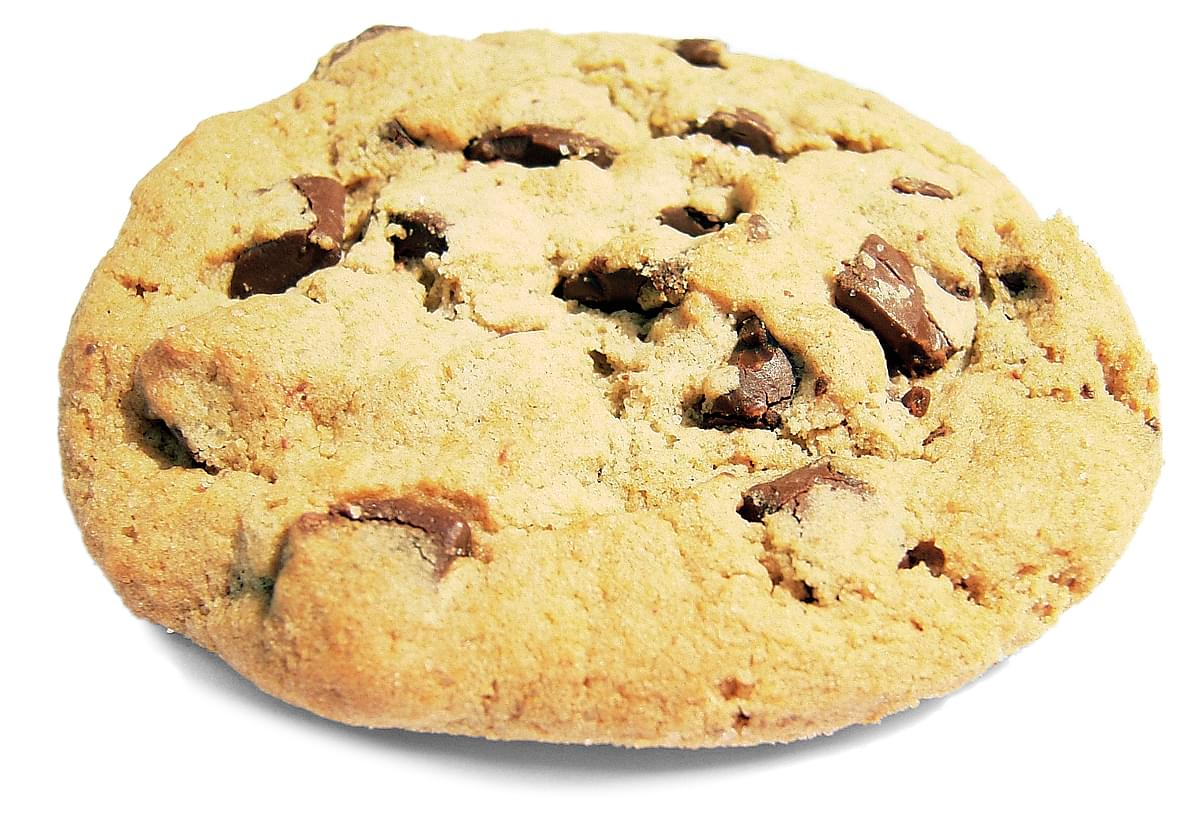
\includegraphics[scale=0.15]{img/cookie.jpg}
            \end{center}
        \end{frame}
        \begin{frame}{label=cookies}
            \frametitle{Les cookies}
            \begin{center}
                \begin{itemize}
                    \item Mini text stocké dans votre navigateur ne pouvant être lu que par le site qui l'a déposé.
                    \item En y laissant un identifiant un site peut facilement vous reconnaître lors de vos visites et reconstituer votre historique sur ce site.
                    \item Les annonceurs utilisent cette pratique pour tracker à l'échelle de plusieurs sites, ce sont des tierces parties.
                \end{itemize}
            \end{center}
        \end{frame}
        \begin{frame}{label=statistiques}
            \frametitle{Les statistiques}
            \begin{center}
                \begin{itemize}
                    \item Pour connaître son audience, un site doit collecter des informations techniques diverses.
                    \item Google et son service analytics est très largement utilisé (54\%) pour collecter ces données.
                    \item Ce qui implique que toutes les visites effectuées sur ces sites sont aussi connues de Google.
                \end{itemize}
            \end{center}
        \end{frame}
        \begin{frame}{label=boutons}
            \frametitle{Les boutons de partage}
            \begin{center}
                \begin{itemize}
                    \item Les réseaux sociaux proposent souvent des boutons pour partager le contenu d'une page.
                    \item Lors du chargement du bouton sur la page, celui-ci collecte également des statistiques sur votre visite.
                    \item Les sites comme Facebook et Twitter peuvent ainsi reconstituer une part très importante de votre historique.
                \end{itemize}
            \end{center}
        \end{frame}
    \subsection{Nouvelles techniques}
        \begin{frame}{label=fingerprinting}
            \frametitle{Le fingerprinting}
            \begin{center}
                \begin{itemize}
                    \item La défense contre les systèmes évqués précedemmen étant trop aisée pour l'utilisateur, les trackers ont développés de nouvelles techniques.
                    \item Le fingerprinting consiste à vous identifier de façon uniqe avec à votre configuration (matérielle et logiciel).
                    \item Pour se défendre, ces systèmes reprennent souvent des fonctionnalités légitimes afin de ne pas être bloquées par l'utilisateur.
                \end{itemize}
            \end{center}
        \end{frame}
        \begin{frame}{label=evercookies}
          \frametitle{Ever cookies}
            \begin{center}
                \begin{itemize}
                    \item Les cookies étant \textit{trop} facilement contrôlables, les trackers développent des techniques plus ou moins évoluées pour qu'ils restent.
                    \item Augmanter la durée de vie, utiliser les cookies Flash, respawn les cookies entre eux, dissimuler leur nature...
                    \item Do Not Track réduit de 2,6\% la synchronisation.
                    \item Seul le Tor browser est efficace à 100\% contre les ever cookies
                \end{itemize}
            \end{center}
        \end{frame}
        \begin{frame}{label=partage}
          \frametitle{Partage d'informations (Top 3000 Alexa --- 2014)}
            \begin{center}
                \begin{itemize}
                    \item Le nombre de domaines capables de recouvrir plus de 40\% de l'historique en se basant sur des cookies de tout type est de \textbf{2}.
                    \item En partageant leurs informations ce chiffre passe à \textbf{161} selon estimation modeste (partage avec un unique tracker à la fois).
                    \item Cette pratique permet à un grand nombre d'entreprise d'avoir un accès conséquent à votre historique.
                \end{itemize}
            \end{center}
        \end{frame}
\end{document}
